% !TeX document-id = {91124dfd-b11a-4cfa-8e46-7efa01057d4d}
% =========================================================================
%
%
% =========================================================================
% !TeX TXS-program:compile = txs:///pdflatex/[--shell-escape]
\documentclass[aspectratio=1610]{beamer}

% ========================= Theme =========================================
\usetheme{CambridgeUS}
\usecolortheme{default}

% ========================= Packages ======================================
\usepackage{calc}
\usepackage{tikz}
\usetikzlibrary{arrows,
arrows.meta,
calc,
chains,
quotes,
positioning,
shapes,
shapes.geometric}
\usepackage{graphicx}
\usepackage{graphics}
\usepackage{pgfplots}
\pgfplotsset{width=7cm,compat=1.17}

%% ========================== Coding snippets =============================
% Default fixed font does not support bold face
\usepackage{minted}

% ========================= Infor on authors ==============================
\title{Intro to Python --- SMM692}
\subtitle{Getting Started with Python}
\author{Simone Santoni}
\institute{Bayes Business School}
\date{MSc Pre-Course Series}

% ============================ Colors =====================================
\definecolor{base_c}{rgb}{0.6,0,0}
\definecolor{comp_c}{rgb}{0.09803921568627451, 0.6901960784313725, 0.7529411764705882}
\definecolor{tri_1}{rgb}{0.09803921568627451, 0.7686274509803922, 0.19215686274509805}
\definecolor{tri_2}{rgb}{0.19215686274509805, 0.09803921568627451, 0.7686274509803922}

% ========================= TOC  ==========================================
\AtBeginSubsection[]
{
    \begin{frame}
        \frametitle{Outline}
        \tableofcontents[currentsection,currentsubsection]
    \end{frame}
}

% ========================= Document  ====================================
\begin{document}

\begin{frame}
	\titlepage
\end{frame}

\begin{frame}{Outline}
	\tableofcontents
\end{frame}

% ------------------------- Background -----------------------------------

\section{Installing Python}

\subsection{Options}

\begin{frame}[c]{Option 1: Official Installer}
	\begin{figure}
		\includegraphics[width=0.75\textwidth]{images/official_installer.png}
	\end{figure}
\end{frame}

\begin{frame}[c]{Option 2: Anaconda Distro (Preffered Way)}
	\begin{figure}
		\includegraphics[width=0.75\textwidth]{images/anaconda_distro.png}
	\end{figure}
\end{frame}

\subsection{Installation Procedure for Anaconda}

\begin{frame}[c]{Steps}
	\begin{enumerate}
		\item Downaload the installer for your operating system (unless you have a very old machine running Win, go for the 64-Bit version)
		\item Run the installer
		\begin{itemize}
			\item For Linux: navigate to the folder where you have downloaded the installer as per step 1, open a shell session, then run \texttt{\$ bash ./Anaconda3-XXXX.XX-Linux-x86-64.sh}
			\item For Win and Mac OS: just run the graphical installer downloaded in step 1
		\end{itemize}
		\item Accept the terms proposed by the Anaconda people to use their software, comprising Python, the \texttt{conda} package manager, and a bundle of modules for data science
		\item That's it!
		\begin{itemize}
		\item For Linux users: if you accepted the default installation options, an environmental variable has been created either in your \texttt{.bashrc} or \texttt{.zshrc}. That means you can access the various pieces of software included in the Anaconda installation (e.g., Anaconda Navigator) from a shell session
		\item For Win and Mac OS users: the various pieces of software included in the Anaconda installation are available from the menu of your system
		\end{itemize}
	\end{enumerate}
\end{frame}

\section{The Anaconda Distribution}

\subsection{Distinctive Features}

\begin{frame}[c]{How is the Anaconda Distro Different?}
	\begin{itemize}
		\item Anaconda is `battery-included' --- it comes with a humongous number of modules for data science
		\begin{itemize}
			\item If you use the official Python installation, then you have to install the modules you need on your own!
		\end{itemize}
		\item  Anaconda is a bundle of various pieces of software:
		\begin{itemize}
			\item \texttt{conda} is the Swiss army knife to manage Python modules and environments
			\item \texttt{anaconda-navigator} is the graphical interface from within to access Python IDEs and related desktop/web applications
		\end{itemize}
	\end{itemize}
\end{frame}

\subsection{The Bundle of Applications}

\begin{frame}[c]{What Software Can I Access from Anaconda Navigator?}
%	\begin{itemize}
%		\item DataSpell
%		\item Datalore
%		\item IBM Watson Studio Cloud
%		\item JupyterLab
%		\item Jupyter
%		\item Qt Console
%		\item Spyder
%		\item VS Code
%		\item GlueViz (for data viz)
%		\item Orange (a point-and-click user interface for Python)
%		\item PyCharm 
%		\item RStudio (the popular IDE for R)
%	\end{itemize}
	\begin{figure}  
		\includegraphics[width=1\textwidth]{images/anaconda_navigator}
	\end{figure}
\end{frame}

\section{How Python Runs Programs}

\begin{frame}[c]{Python as a Language and Interpreter}
	\begin{itemize}
	\item Typically, we refer to Python as a programming language
	\item However, Python is also a software package called an interpreter
	\begin{itemize}
		\item An interpreter is a kind of program that executes other programs
		\item When you write a Python program, the Python interpreter reads your program and carries out the instructions it contains
		\item In effect, the interpreter is a layer of software logic between your code and the computer hardware on your machine
	\end{itemize}
	\end{itemize}
\end{frame}

\begin{frame}[c]{Python Execution Model}
	\begin{columns}
		\begin{column}{0.6\textwidth}
			\begin{itemize}
				\item When you instruct Python to run your script (e.g., `script.py'), there are a few steps the interpreter carries out before your code actually starts crunching away
				\item First, the code is compiled to something called `byte code'
				\begin{itemize}
					\item This step happens behind the scenes (there is nothing to do for the programmer!)
      					\item A file called `script.pyc', automatically generated, contains the translation of your code into lower-level code instructions
				\end{itemize}
				\item Then, the compiled code is routed to something called a `Python Virtual Machine' (PVM)
				\begin{itemize}
					\item This step is hidden to the programmer like the previous one
					\item Mainly, it iterates through your byte code instructions, one by one, to carry out their operations
			\end{itemize}
				\end{itemize}
		\end{column}
		\begin{column}{0.4\textwidth}
			\centering
			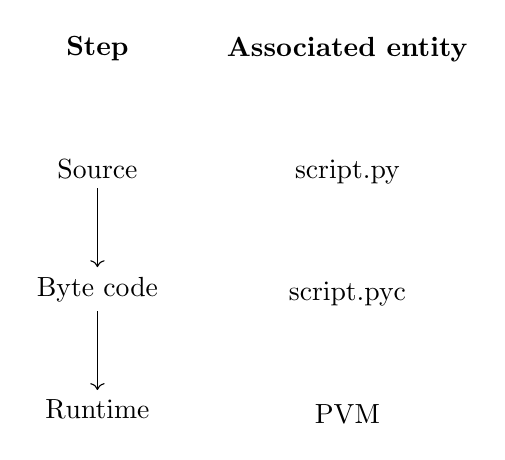
\begin{tikzpicture}[
				->
			]
				\node [] (step) {\textbf{Step}};
			        \node [right=of step] (file) {\textbf{Associated entity}}; 
			        \node [below=of step] (source) {Source};
				\node [below=of file, align=right] (sourcef) {script.py};
				\node [below=of source] (byte) {Byte code};
				\node [below=of sourcef, align=right] (bytef) {script.pyc};
				\node [below=of byte] (pvm) {Runtime};
				\node [below=of bytef, align=right] (pvmf) {PVM};
				\path[]
					(source) edge node [] {} (byte)
					(byte) edge node [] {} (pvm);
			\end{tikzpicture}
		\end{column}
	\end{columns}
\end{frame}

\section{How We Run Python Programs}

\subsection{Non-Interactive Approach}

\begin{frame}[fragile]{Script Preparation $\rightarrow$ Script Run}
	\begin{columns}[t]
		\begin{column}{0.45\textwidth}		
		\textbf{Step 1: script preparation}	
		
		\vspace{1em}
		
		The below displayed Python code achieves two things:i) it prints the string object ``Bazinga!'', and ii) it prints the resul of the algebraic operation $4 + 2$. Note that all lines starting with \texttt{\#} are not considered Python code --- instead, they are comments that illustrate/explain the logic of the script.
		
		\rule{\textwidth}{1pt}
		\scriptsize
		\begin{minted}{python}
# Print a string object
print("Bazinga")
# Print the result of an algebraic operation
print(2 + 4)
	    \end{minted}
		\rule{\textwidth}{1pt}
		
		\end{column}
		\begin{column}{0.45\textwidth}
		\textbf{Step 2: script run}	
		
		\vspace{1em}
		
	\begin{figure}
		\includegraphics[width=0.92\textwidth]{images/simple_script}
	\end{figure}
		\end{column}
	\end{columns}
\end{frame}

\subsection{Interactive Approach}

\begin{frame}{Running a Python Shell in the Terminal}
		\begin{figure}
			\includegraphics[width=0.9\textwidth]{images/python_session}
		\end{figure}
\end{frame}

\begin{frame}{Running an IPython Shell in the Terminal}
		\begin{figure}
			\includegraphics[width=0.9\textwidth]{images/ipython_session}
		\end{figure}
\end{frame}

\begin{frame}[t]{Running a Python IDE}

	\begin{columns}[t]
	
	\begin{column}{0.45\textwidth}

	There are plenty of Python IDEs in the market, including:
	
	\begin{itemize}
		\item Colab (online)
		\item IDLE
		\item Datalore (online)
		\item Jupyter/Jupyterlab
		\item PyCharm
		\item Qt Console
		\item Spyder
		\item Thonny
		\item Wing
	\end{itemize}
	
	\end{column}
	
	\begin{column}{0.45\textwidth}
	
	By installing a couple of plugins, the following (advanced) text editors can turn into Python IDEs:
	
	\begin{itemize}
		\item Emacs
		\item Vim/Neovim
		\item VSCode
	\end{itemize}
	
	\end{column}
	
	\end{columns}
\end{frame}

\begin{frame}{Interactive Python Coding with Jupyter}
		\begin{figure}
			\includegraphics[width=0.9\textwidth]{images/jupyter}
		\end{figure}
\end{frame}

\begin{frame}{Interactive Python Coding with VSCode}
		\begin{figure}
			\includegraphics[width=0.9\textwidth]{images/vscode}
		\end{figure}
\end{frame}

\begin{frame}{Interactive Python Coding in Jupyter with VSCode}
		\begin{figure}
			\includegraphics[width=0.9\textwidth]{images/jupyter_in_vscode}
		\end{figure}
\end{frame}

\section{Managing Python Environments}

\subsection{The What and Why of PyEnvs}

\begin{frame}[t]{What is a Python Environment?}
	\begin{columns}[t]
		\begin{column}{0.45\textwidth}
			Step 1: What is a Python Environment?
		\end{column}
		\begin{column}{0.45\textwidth}
			Step 2: Why would I use a Python Environment?
		\end{column}
	\end{columns}
\end{frame}

\subsection{The How of PyEnvs}

\subsection{Creating PyEnvs from the Command Line}

\begin{frame}[c]{}	
\end{frame}

\subsection{Creating PyEnvs using Anaconda Navigator}

\begin{frame}[c]{}	
\end{frame}


\section{Collaborative and Versioning Tools}

\end{document}